\begin{center}
 \textsc{Физбой, 9 класс.}
\end{center}
\vspace{0.01cm}
\hrule
\parindent=0mm

\taskpic{Катушка катится без проскальзывания по горизонтальной
  поверхности, причем скорость конца нити (точка~$A$) горизонтальна и
  равна $v$. На катушку опирается шарнирно закрепленная в точке~$B$
  доска. Внутренний и внешний радиусы катушки равны $r$ и $R$
  соответственно. Определите угловую скорость $\omega$ доски в
  зависимости от угла
  $\alpha$.}{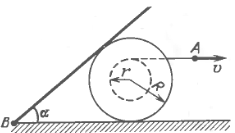
\includegraphics[width=4cm]{fb01.png}}


\task{На тело, движущееся с постоянной скоростью $\vec{v}$, начинает
  действовать некоторая постоянная сила. Спустя промежуток времени
  $\Delta t$ скорость тела уменьшается в два раза. Спустя еще такой же
  интервал времени скорость уменьшается еще в два раза. Определите
  скорость $v_{\mbox{\textit{к}}}$ тела через интервал времени
  $3\Delta t$ с начала действия постоянной силы.}

\taskpic{Для покоящейся системы, изображенной на рисунке, найдите
  ускорения всех грузов сразу после того, как была перерезана
  удерживающая их нижняя нить. Считать, что нити невесомы и
  нерастяжимы, пружины невесомы, масса блока пренебрежимо мала, трение
  в подвесе отсутствует.}{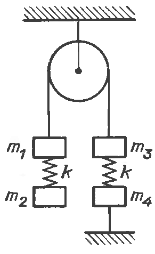
\includegraphics[width=2cm]{fb03.png}}

\task{Вблизи поверхности земли свободно падает тело массой $m$. В
  некоторый момент времени в него попадает (и застревает)
  горизонтально летящая тяжелая пуля массой $M$. Определите время
  падения $t$ тела, если известно, что пуля попала в тело на половине
  пути, а время свободного падения тела с той же высоты равно
  $t_0$. Считать, что масса пули много больше массы тела ($M \gg
  m$). Сопротивлением воздуха пренебречь.}

\taskpic{В ведре находится смесь воды со льдом массой $m = 10\mbox{
    кг}$. Ведро внесли в комнату и сразу же начали измерять
  температуру смеси. Получившаяся зависимость температуры от времени
  $T(\tau)$ изображена на графике. Удельная теплоемкость воды равна
  $c_{\mbox{\textit{в}}} = 4{,}2 \mbox{
    кДж}/(\mbox{кг}\cdot\mbox{К})$, удельная теплота плавления льда
  $\lambda = 340 \mbox{ кДж/кг}$. Определите массу
  $m_{\mbox{\textit{л}}}$ льда в ведре, когда его внесли в
  комнату. Теплоемкостью ведра
  пренебречь.}{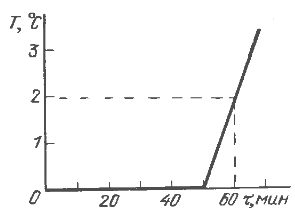
\includegraphics[width=4cm]{fb05.png}}

\taskpic{В схеме, изображенной на рисунке, сопротивления всех
  резисторов одинаковы и равны $R$. Напряжение на клеммах равно
  $U$. Определите силу тока $I$ в подводящих проводах, если их
  сопротивлением можно
  пренебречь.}{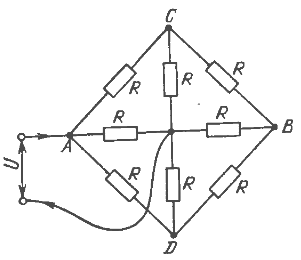
\includegraphics[width=4cm]{fb06.png}}

\setcounter{notask}{1}